\section{Microcontroller Basics}

\subsection{Signalgruppen eines System Bus}

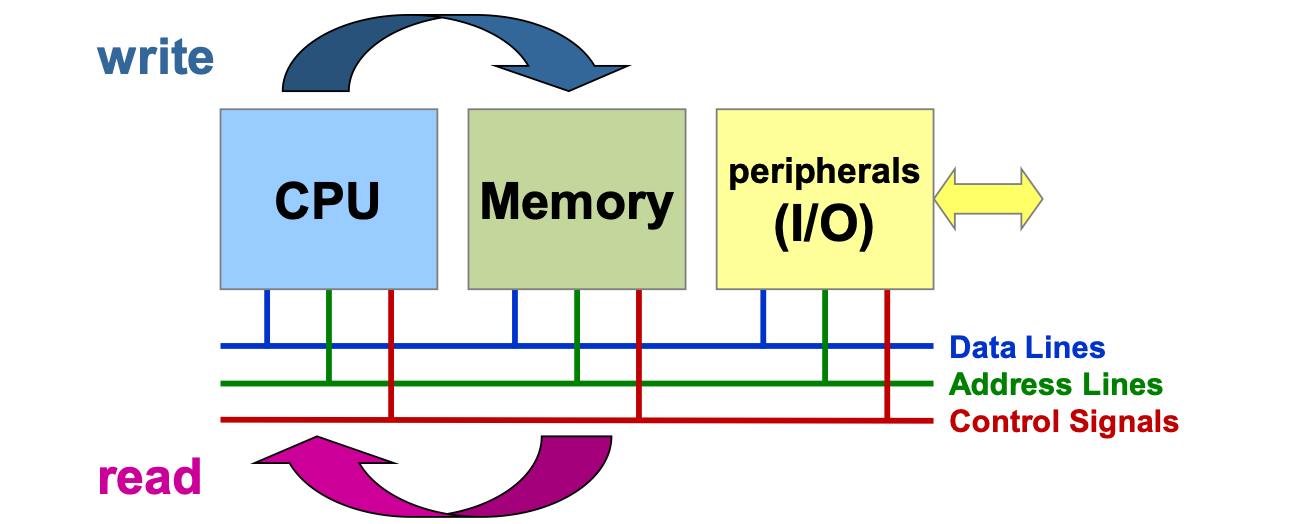
\includegraphics[width=0.3\textwidth]{images/system_bus.png}

\begin{itemize}
    \item \textbf{Address Bus}: Unidirektional (Master $\rightarrow$ Slave), die Anzahl der Adressleitungen bestimmt die Anzahl der adressierbaren Speicherzellen.
    \item \textbf{Data Bus}: Bidirektional, 8, 16, 32 oder 64 Bit parallele Datenverbindungen
    \item \textbf{Control Bus}: Steuerleitungen, die die Kommunikation zwischen Master und Slave steuern.
\end{itemize}

\subsection{Asynchrone vs. Synchrone Datenübertragung}
\subsubsection{Synchrone Datenübertragung}
\begin{itemize}
    \item Master und Slave haben einen gemeinsamen Takt.
    \item CLK Flanke bestimmt die Datenübertragung auf beiden Seiten.
\end{itemize}
\subsubsection{Asynchrone Datenübertragung}
\begin{itemize}
    \item Slaves haben keinen Zugriff auf den Takt des Masters.
    \item Control Signale haben Taktinformationen für die synchronisierung.
\end{itemize}

\subsection{Tri-State Logik}
Wenn ein Gerät ein logisches 1 (Vcc) und ein anderes Gerät ein logisches 0 (GND) ausgibt, entsteht ein Kurzschluss. Um dies zu verhindern, wird die Tri-State Logik verwendet. Ein Gerät kann den Bus entweder auf 0, 1 oder hochohmig schalten. Der hochohmige Zustand wird durch ein drittes Signal (Enable) gesteuert.
\subsubsection{CMOS Tri-State Inverter}
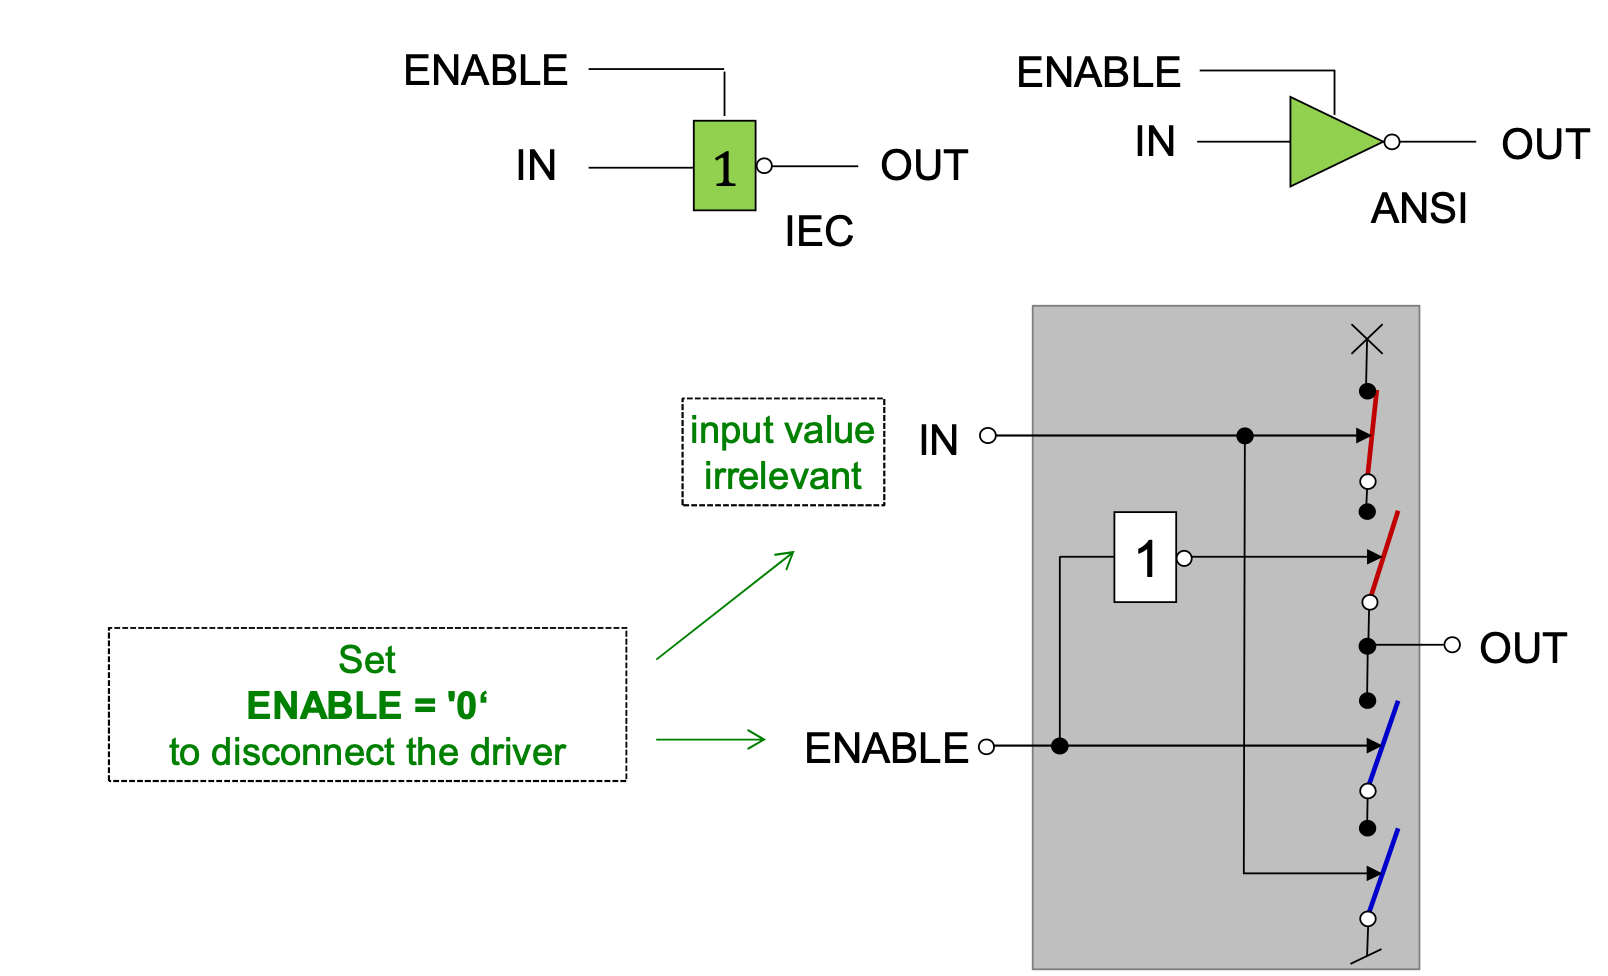
\includegraphics[width=0.3\textwidth]{sections/images/cmos_tri.png}\\
Wenn $EN = 0$, dann ist der Ausgang hochohmig. Wenn $EN = 1$, dann ist der Ausgang das Inverse des Eingangs.

\subsection{Timing Diagramm Notation}
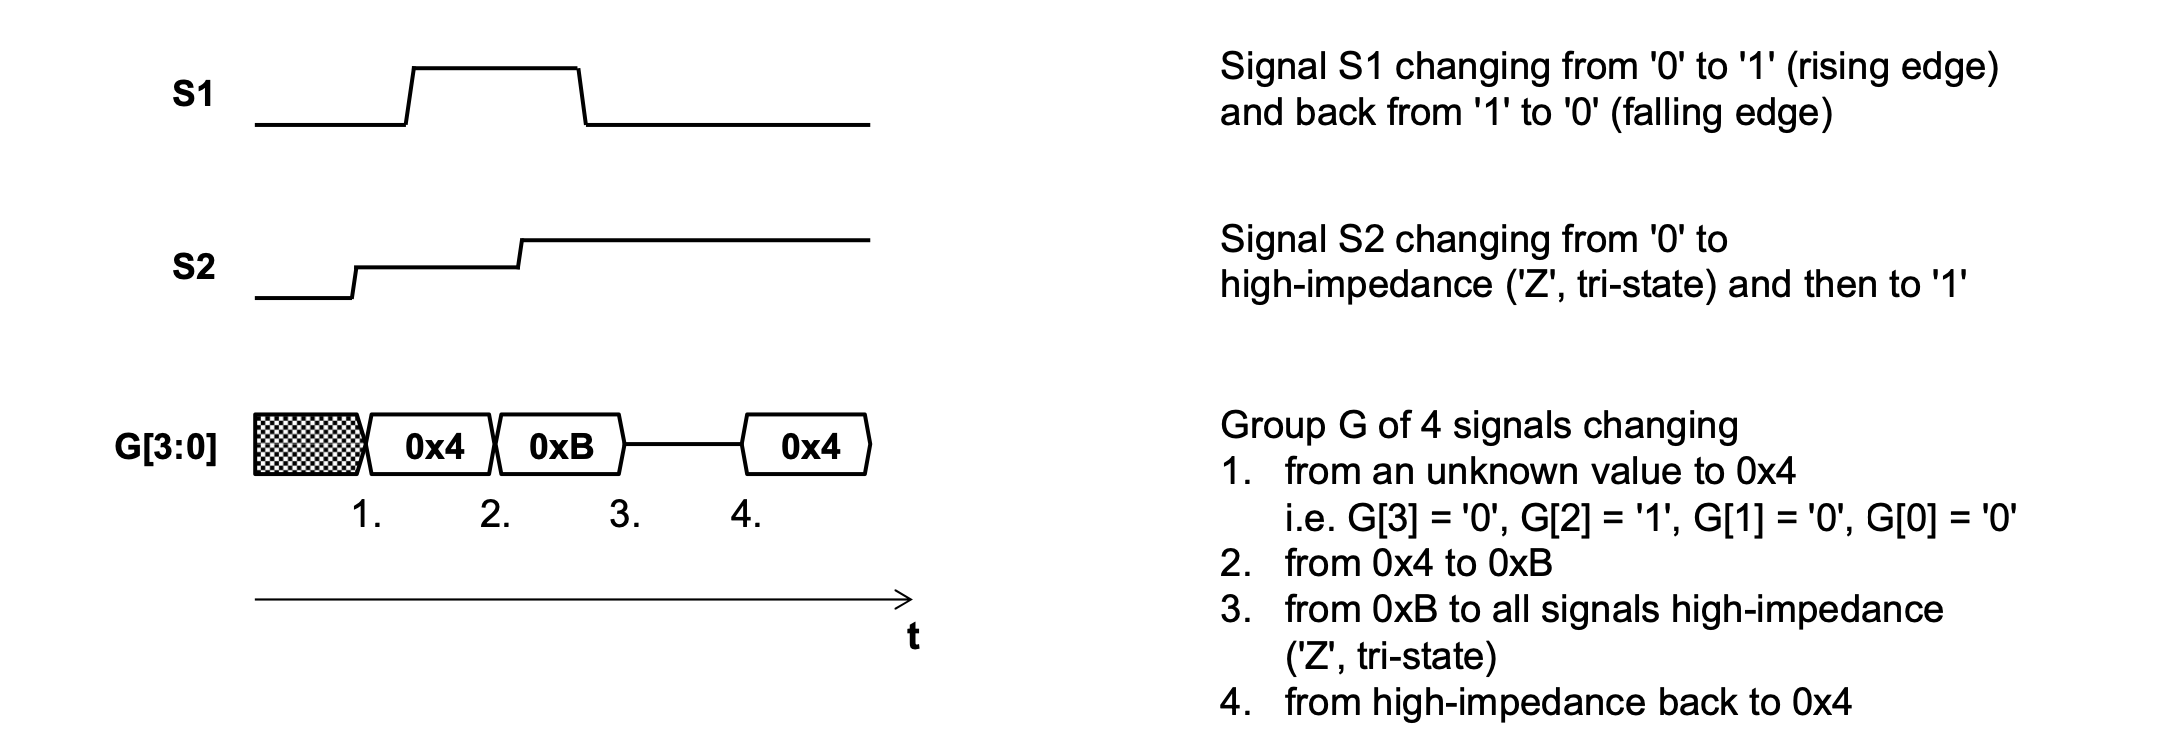
\includegraphics[width=0.3\textwidth]{sections/images/timing_diagram.png}

\subsection{Block Diagramm}
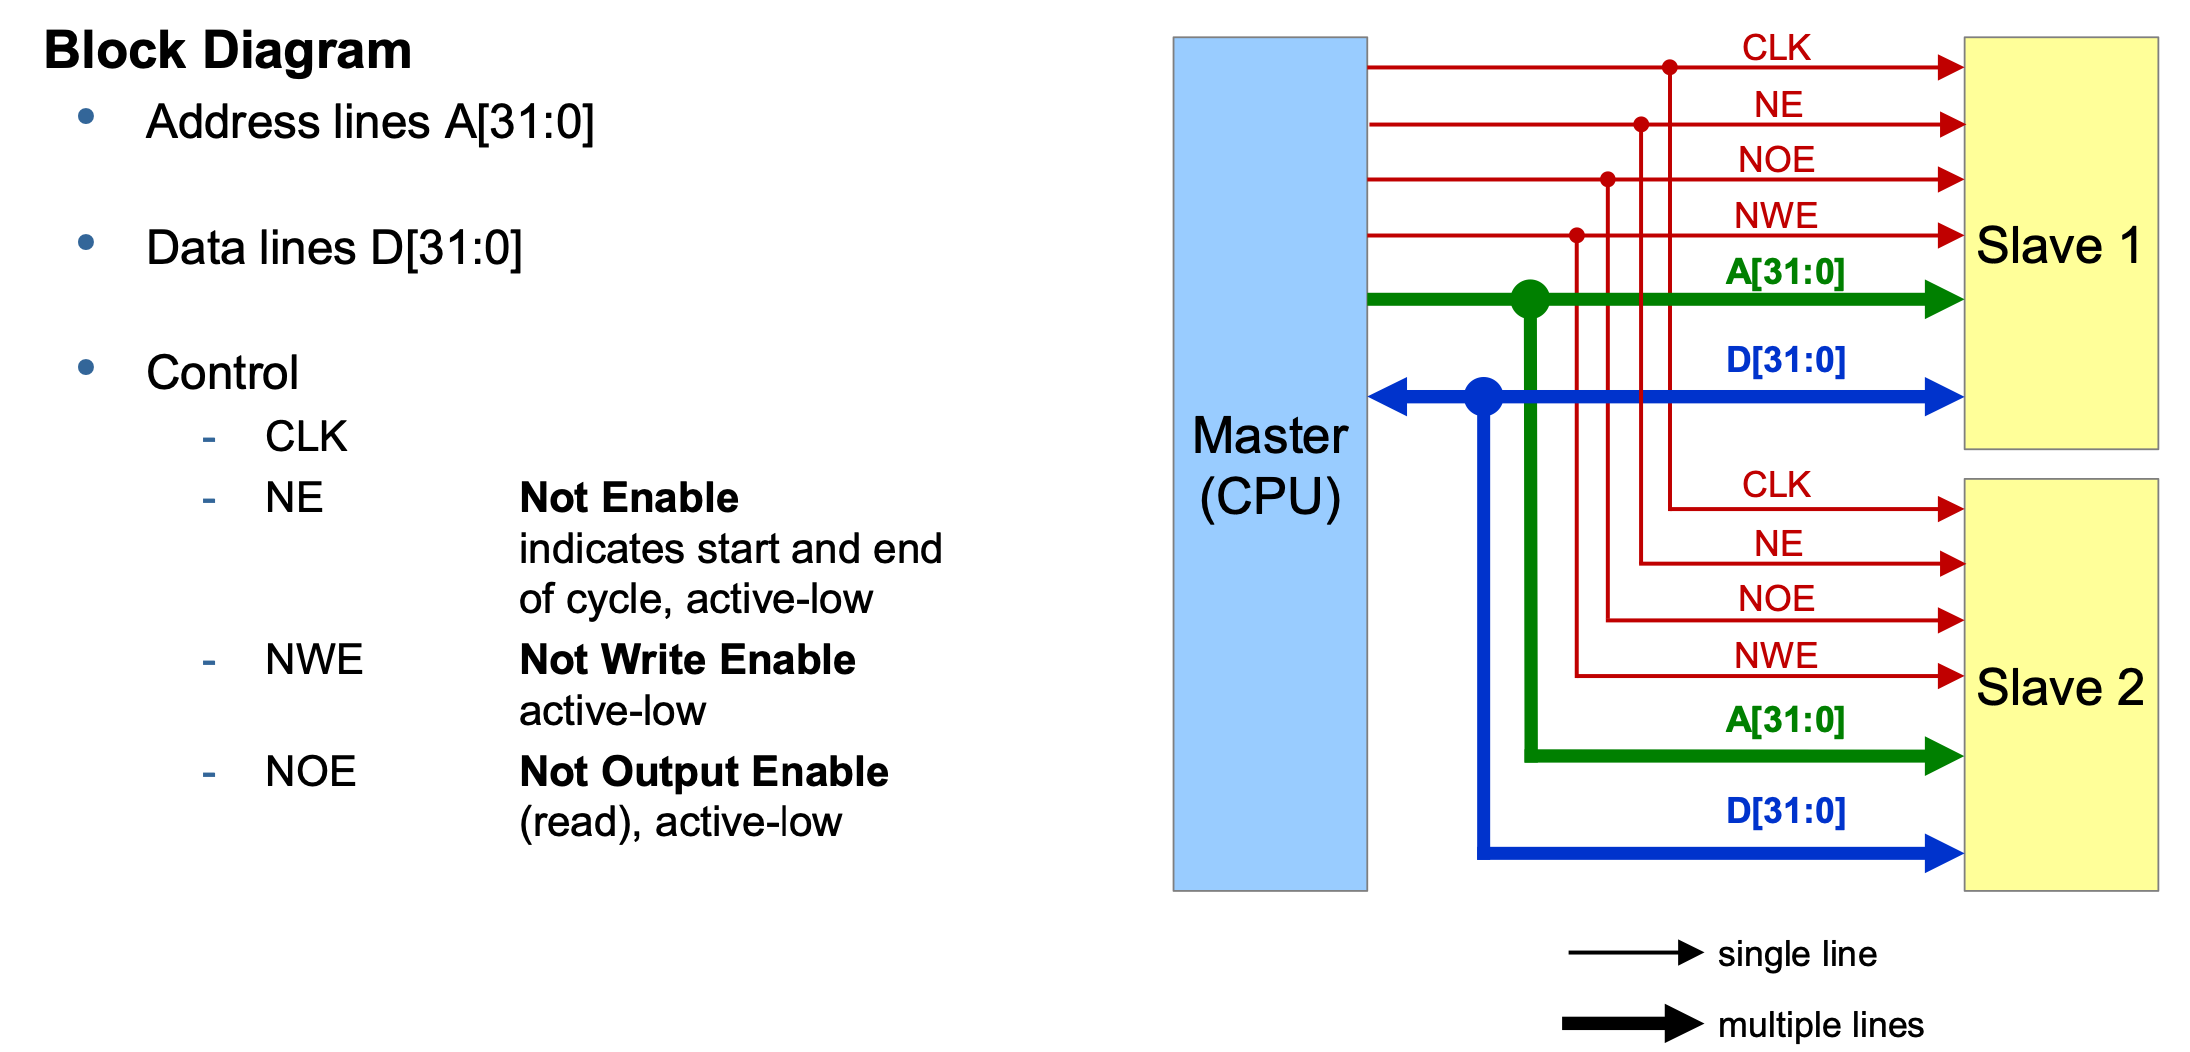
\includegraphics[width=0.3\textwidth]{sections/images/block_diagram.png}

\subsubsection{Beispiel: Schreiboperation}
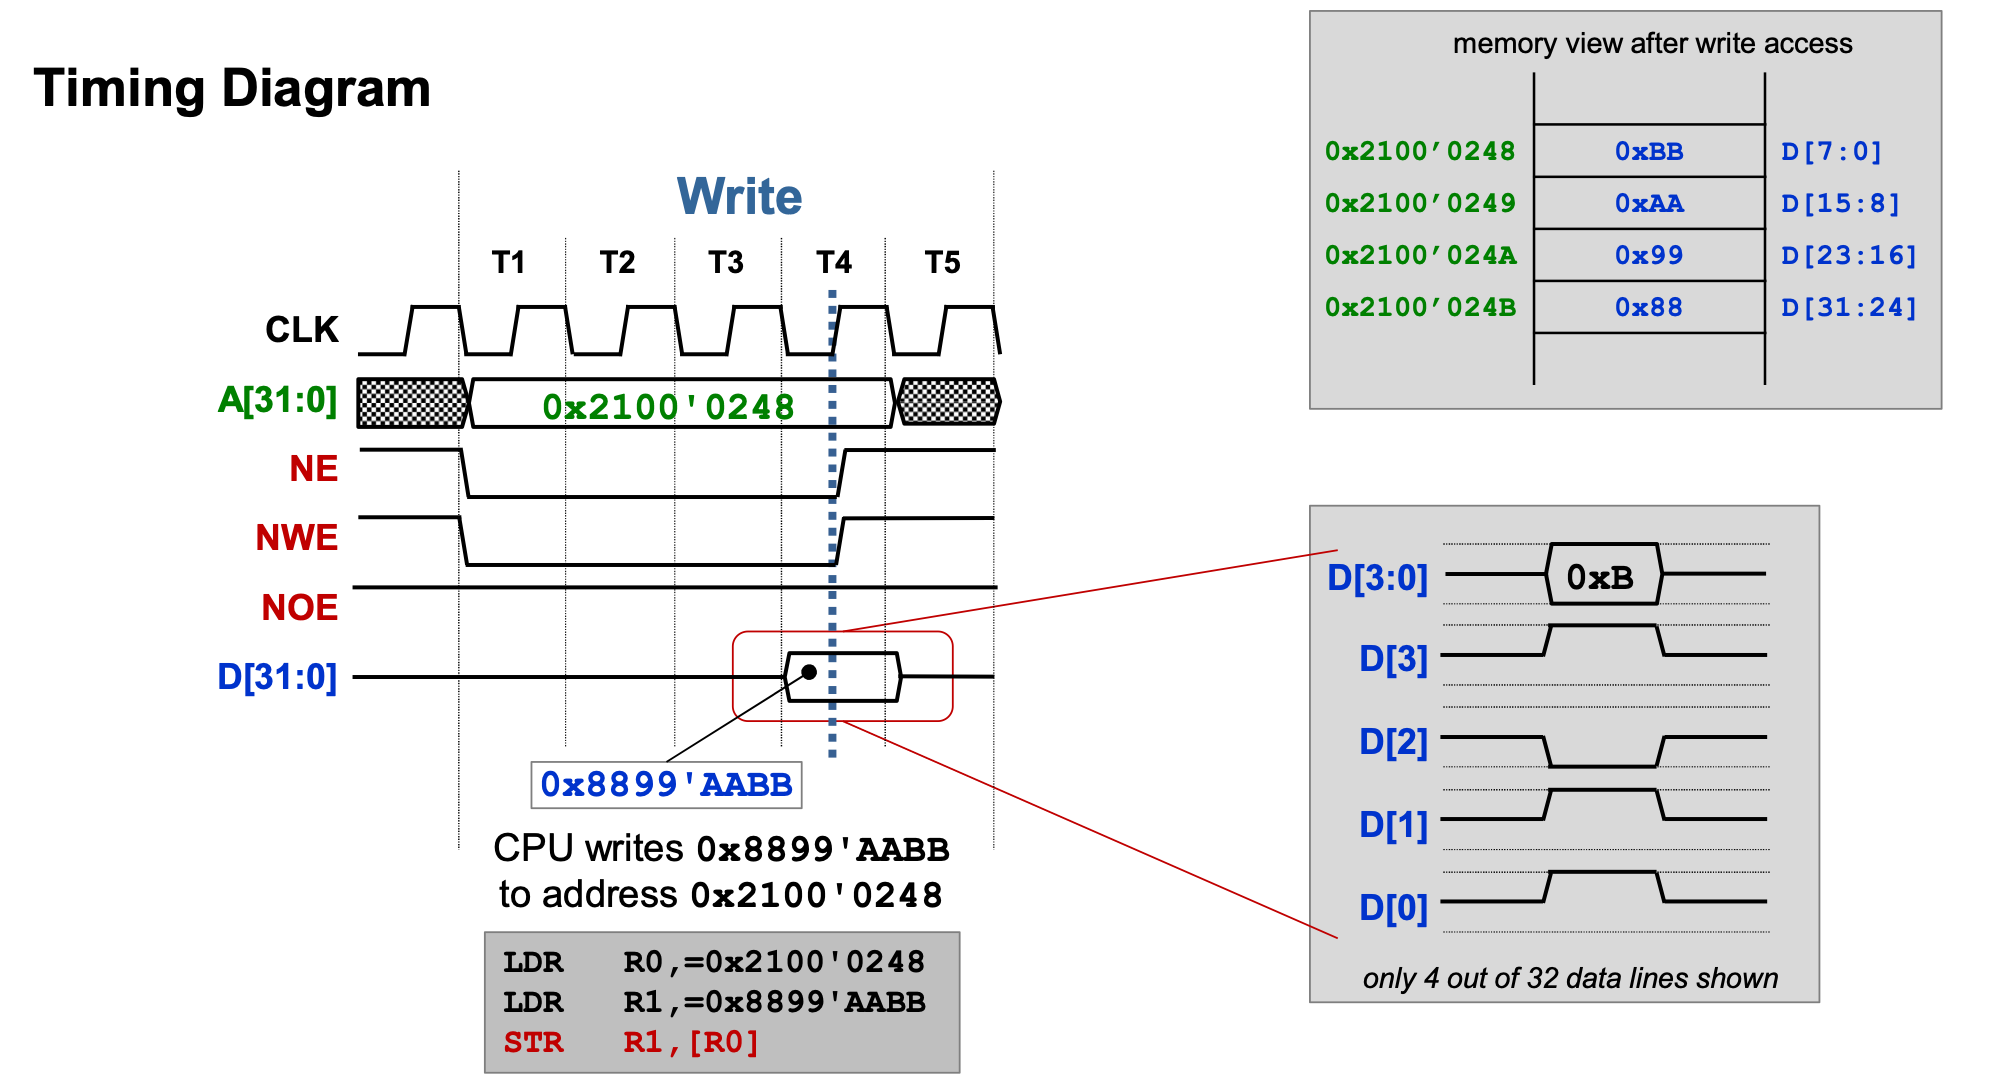
\includegraphics[width=0.3\textwidth]{sections/images/schreiboperation.png}

\subsection{Control- und Status-Register}
\subsubsection{Control Register}
\begin{itemize}
    \item Steuerung der Slaves (von CPU)
    \item CPU schreibt in Register Bit
    \item Slave liest Register Bit
    \item Beispiel: LED interface (on/off)
\end{itemize}
\subsubsection{Status Register}
\begin{itemize}
    \item CPU kann Status des Slaves abfragen
    \item Slave schreibt Status in Register Bit
    \item CPU liest Register Bit
    \item Meistens read-only
    \item Beispiel: Daten Byte auf serial interface empfangen
\end{itemize}

Achtung: Das selbe Register kann sowohl Control- als auch Status-Register sein, je nachdem ob die CPU schreibt oder liest.

\subsection{Wait States}
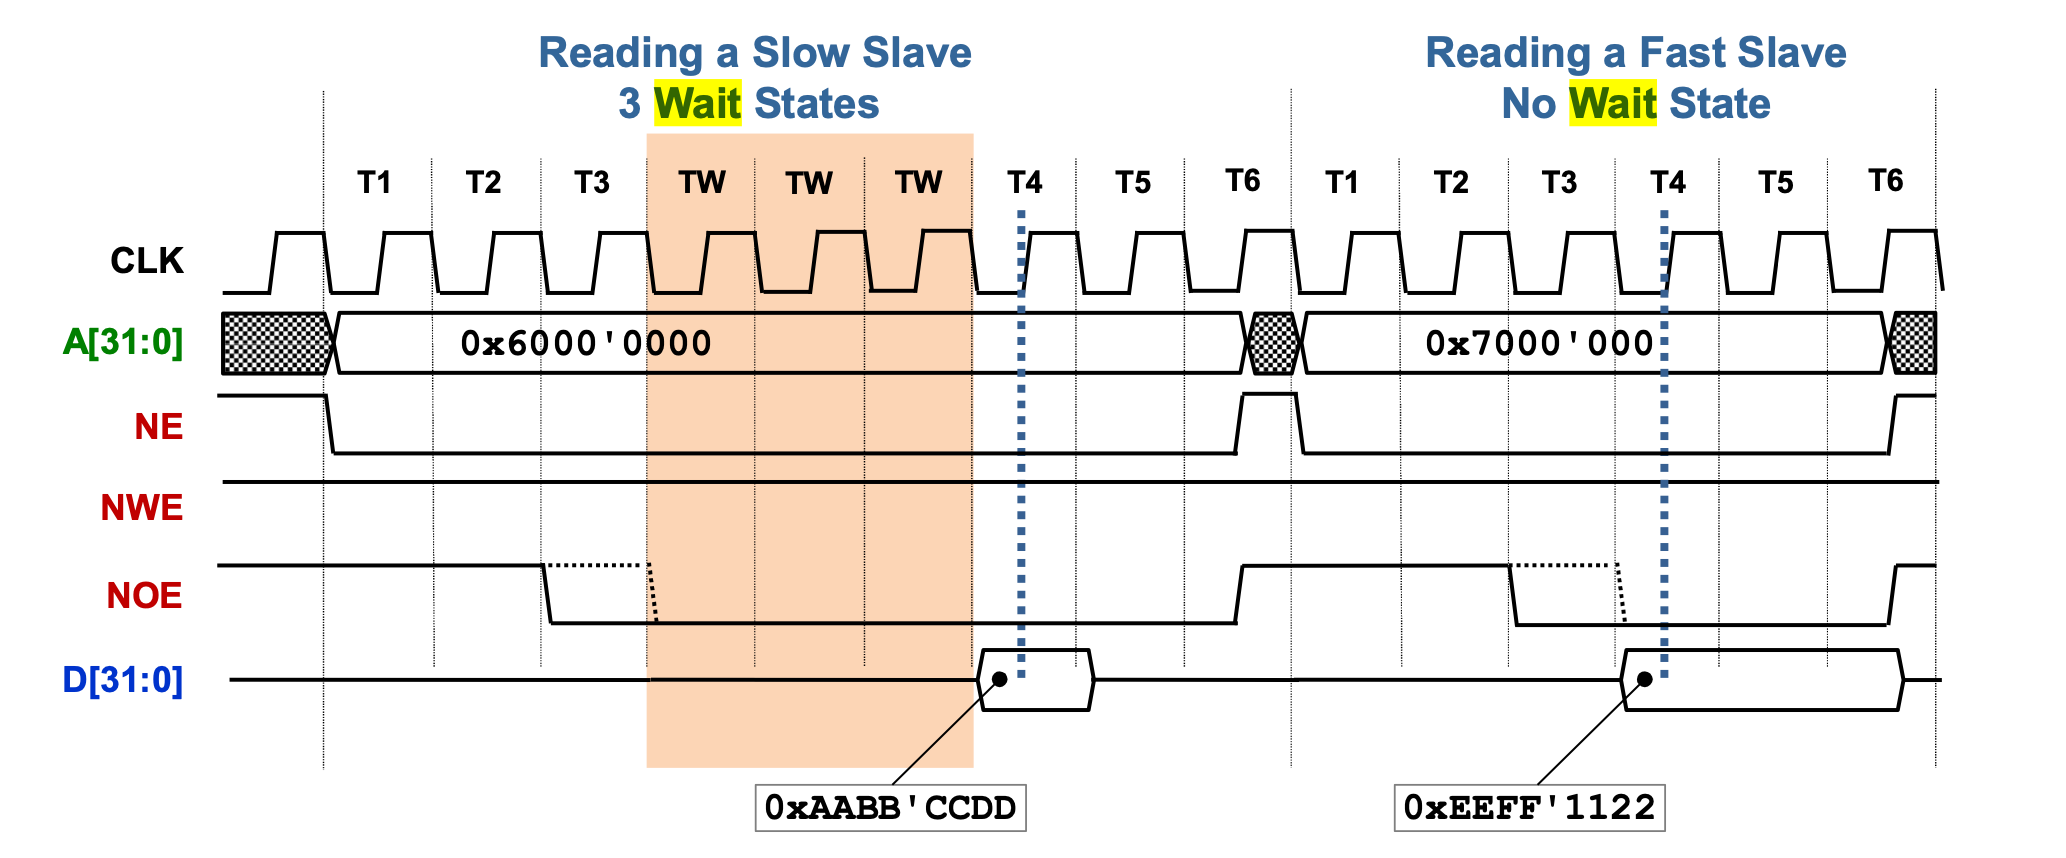
\includegraphics[width=0.3\textwidth]{sections/images/wait_state.png}
\begin{itemize}
    \item Wartezyklen, die eingefügt werden, um die Geschwindigkeit von Master und Slave anzugleichen.
    \item Wird benötigt, wenn der Slave langsamer ist als der Master.
    \item Wird benötigt, wenn der Slave mehr Zeit benötigt, um Daten zu verarbeiten.
    \item Individuelle wait states können auf der CPU (bus interface unit) programmiert werden.
    \item Andere Möglichkeit: Der Slave sendet ein "ready" Signal an den Master, wenn er bereit ist.
\end{itemize}

\subsection{Full vs. Partial Address Decoding}
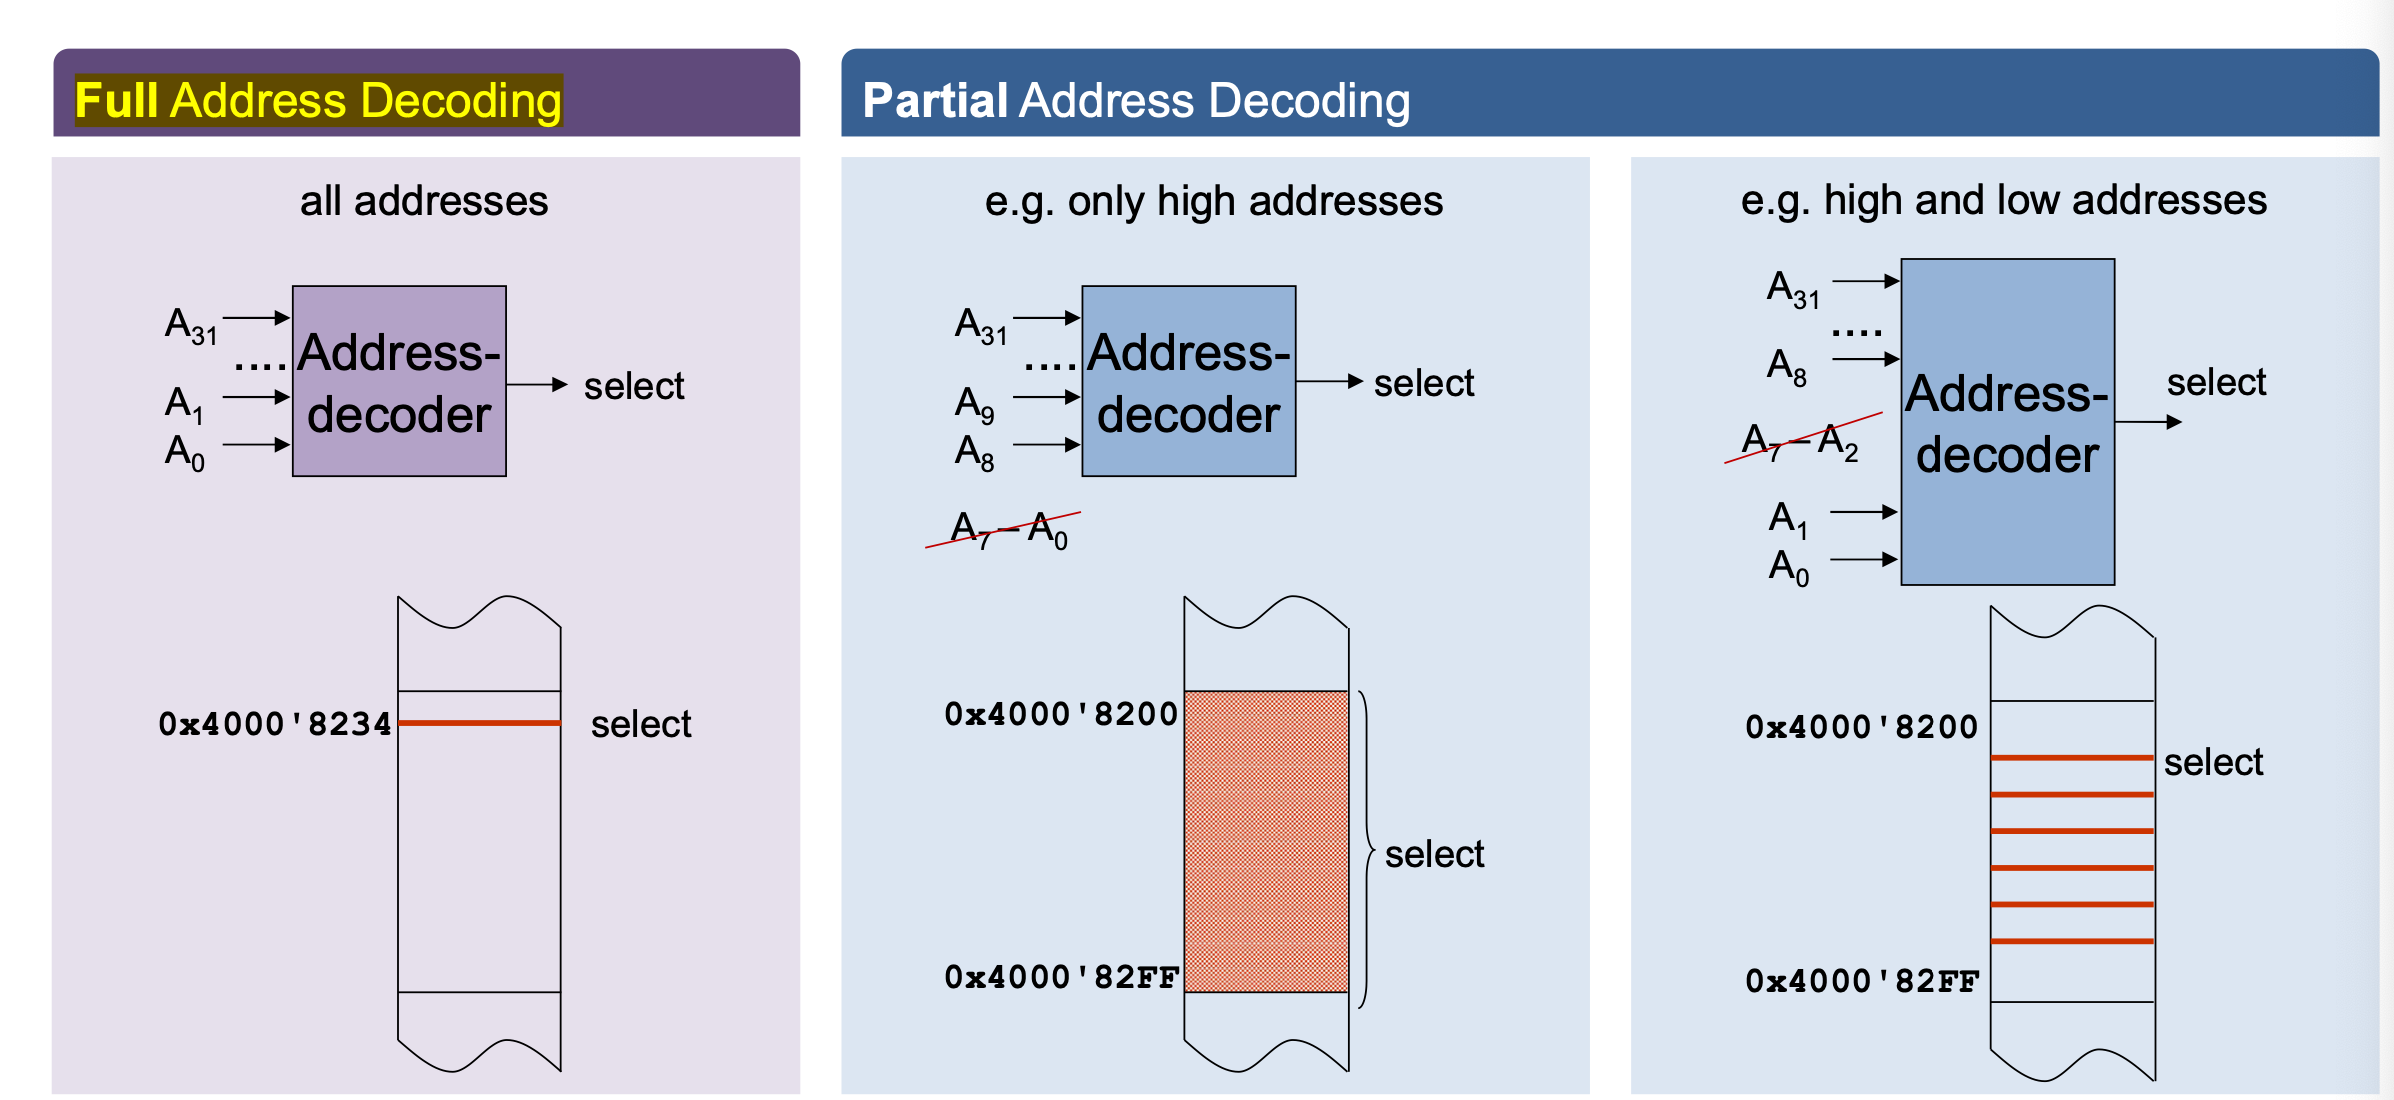
\includegraphics[width=0.3\textwidth]{sections/images/full_partial_address_decoding.png}
\subsubsection{Full Address Decoding}
\begin{itemize}
    \item Alle Addressleitungen werden dekodiert
    \item Alle Control Register können an genau einer Adresse angesprochen werden
    \item 1:1 Mapping von Addressen zu Control Registern
\end{itemize}
\subsubsection{Partial Address Decoding}
\begin{itemize}
    \item Nur ein Teil der Addressleitungen wird dekodiert
    \item Mehrere Control Register können an einer Adresse angesprochen werden
    \item n:1 Mapping von Addressen zu Control Registern
\end{itemize}

\subsection{Control Register in C ansteuern}
\subsubsection{Qualifier Volatile}
Der Compiler darf keine Annahmen über den Wert der Variable machen, da dieser sich jederzeit ändern kann. Der Compiler darf die Variable nicht optimieren. Keyword: \texttt{volatile}
\subsubsection{Pointer auf Register}
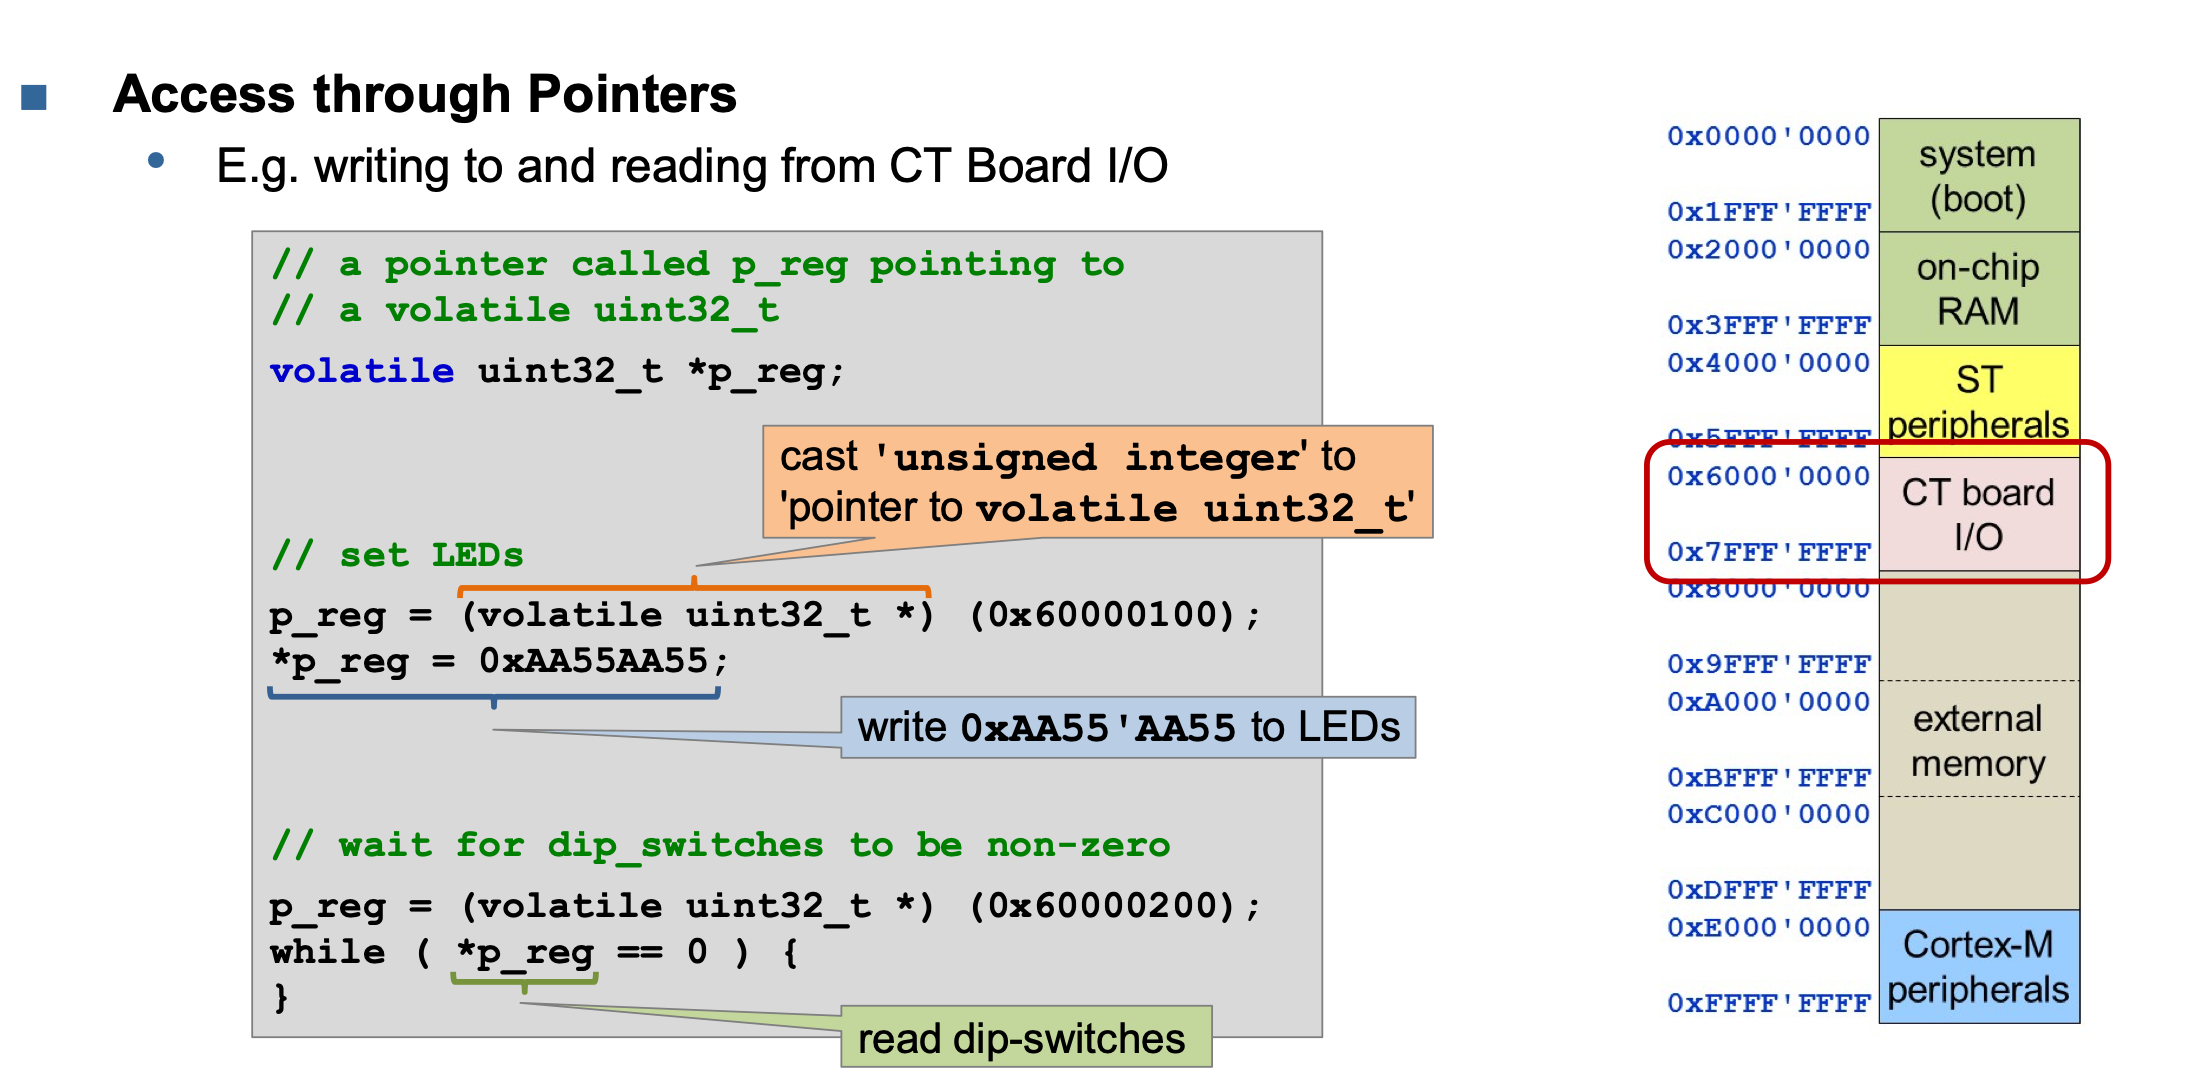
\includegraphics[width=0.3\textwidth]{sections/images/pointer_c.png}
\subsubsection{Preprocessor Macros}
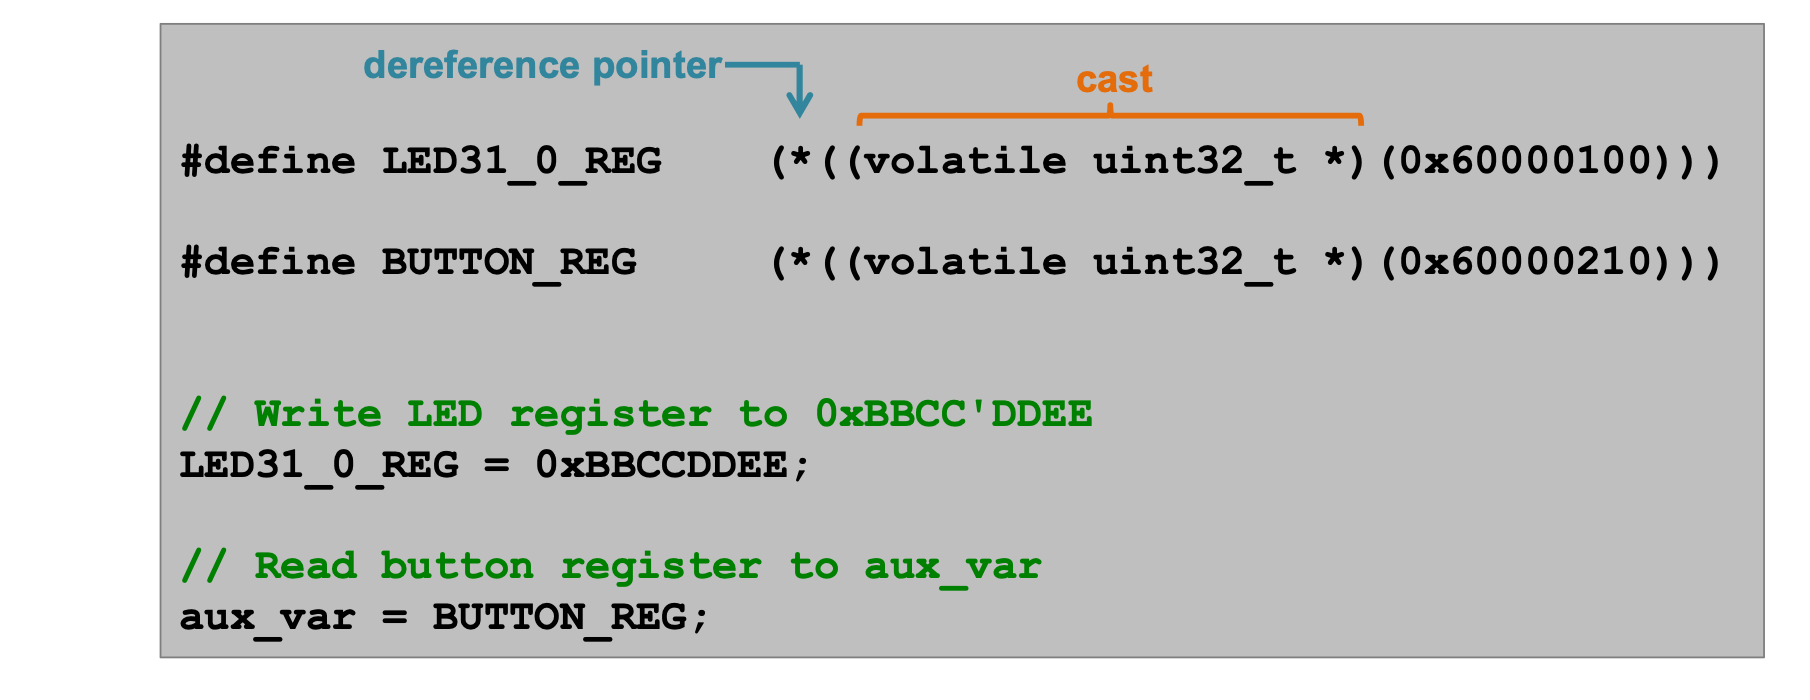
\includegraphics[width=0.3\textwidth]{sections/images/preprocessor_c.png}